\begin{figure}[h!]
\centering
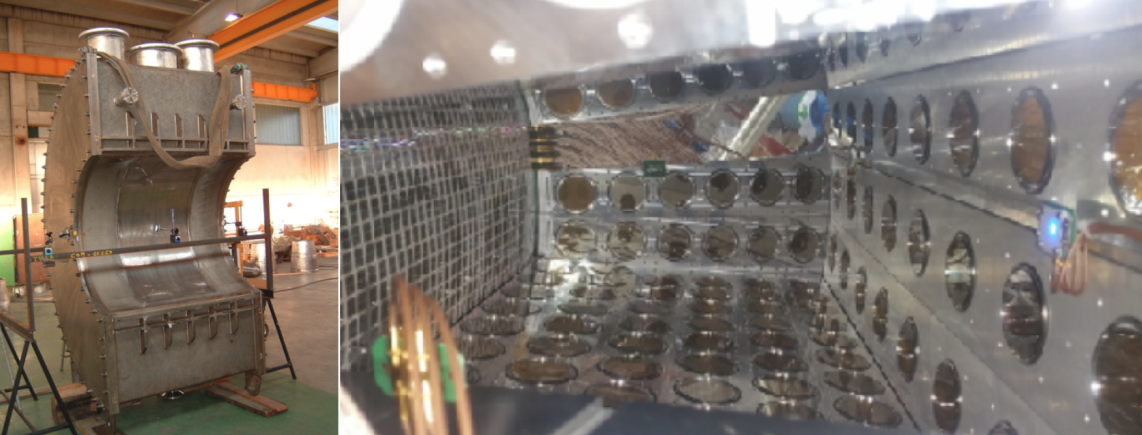
\includegraphics[scale=.4]{sections/figures/calo.meg.png}\vspace{3mm}\\
\caption{placeholder MEG, Toshiyuki please provide nice pictures}
\label{fig:calo.meg}
\end{figure}

One  concept for the new experiment is based on a liquid xenon (LXe) scintillating calorimeter for detection of positrons and gammas from pion decays. A 25-30 X$_o$ thick LXe scintillation calorimeter read out with fast-digitized SiPMs
has extraordinary properties including high light output (65k photons per MeV deposit), fast timing
($\sim$ ns decay time), and near complete containment of EM showers, making it suitable for this
application. Based on experience with the MEG LXe photon calorimeter \cite{Baldini} (see fig.~\cite{fig:calo.meg}) it is reasonable to
expect 1-2 \% energy resolution (comparable to \cite{Aguilar-Arevalo3} ), 50 ps timing resolution, and transverse (depth) position resolution of 5 mm 
(6 mm). Our Japanese collaborators are world experts on this detector technology. They have established basic LXe properties and suitable
simulation codes, conditioned on the MEG detector response, which will be critical for scaling up the design. \todo{Toshiyuki, Toshi, Sathoshi, that's just a placeholder for your part}
Due to the fast scintillation response of LXe (orders of magnitude faster than the NaI(Tl) and
pure CsI used in \cite{Aguilar-Arevalo1, Aguilar-Arevalo2} and \cite{Pocanic1, Pocanic2}), a low-energy pion beam rate of several 10$^5$ Hz can be used, more than an order of magnitude greater than previous experiments, which were impacted by pulse pile-up effects. Systematic effects would be reduced due to the highly uniform response and depth of the total absorption LXe calorimeter. 

\begin{figure}[h!]
\centering
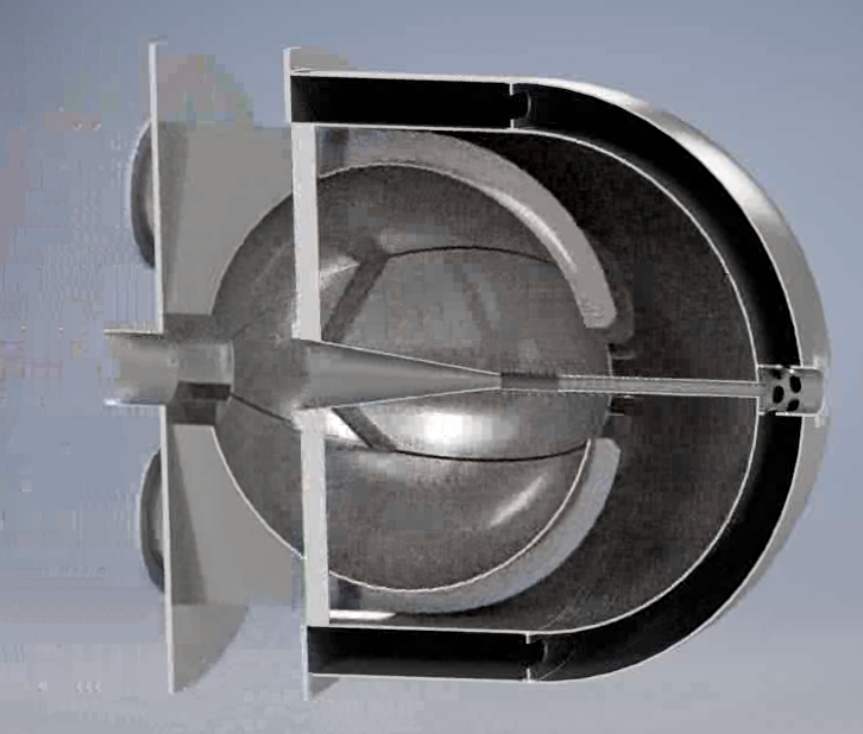
\includegraphics[scale=.4]{sections/figures/calo.Xe.png}
\caption{placeholder  \nexp\ CALO }
\label{fig:calo.Xe}
\end{figure}

\begin{table}
\center
\begin{tabular}{llll}
\hline
\hline
 parameter  &  	value		& 	unit		&  comment \\
\hline
Xe shell radius				&		&		&		\\
Xe volume					&		&		&		\\
Xe weight					&		&		&		\\
Xe entrance window radius	&		&		&		\\
vacuum window radius		&		&		&		\\
\hline
SiPM sensor size			&		&		&		\\
\# sensors					&		&		&		\\
\hline
\hline
\end{tabular}
\caption{Basic \nexp\ CALO parameters. \todo{Xe Ryan, SiPM Toshi, Satoshi et al}}
\label{tab:detpar}
\end{table}
The current conceptional design of the \nexp\ CALO draws on the experience of MEG, but involves several new features, see fig.~\ref{fig:calo.Xe} and Table~\ref{tab:detpar}.
\todo{Ryan: please continue}


